\section{Electroweak probes}
\label{sect:pas:ew}
%- Utility of penetrating probes
%- ALICE low pT photons measuring QCD temperature (cf. PHENIX)
%- Expected scaling of hard probes in A+B (nuclear thickness)
%- PDFs and nPDFs, calculation schemes (LO vs. NLO), codes
%- Z bosons (CMS first result cf. QCD), ATLAS Z centrality & rapidity
%- W (CMS published - can i compare to ATLAS prelim on a plot?)
%- Photon (CMS 2010, ATLAS prelim 2011?)

While a primary topic in the study of heavy ion collisions is the modification
of jets in the hot and dense nuclear medium, typical analyses of
hard processes have assumed that the
structure of a nucleon in a nucleus-nucleus collision is quantitatively the
same as one in a nucleon-nucleon collision.
From analyses of lepton-nucleus deep inelastic scattering data,
it is known that cross sections do not scale linearly with the number of nucleons,
as might be expected simply from the availability of scattering centers.
The deviations from this scaling are referred to generally as ``nuclear shadowing'',
and are typically shown as a function of Bjorken $x$ for different ranges in the
hardness scale $Q^2$.
The region around $x \sim 0.1$ corresponds to the valence quark region for a standard
nucleon, and this is usually enhanced.  The region above this, $x \geq 0.2$ is typically
suppressed (the so-called ``EMC effect''), while the region below $x << 0.1$ is also
suppressed down to very small values of $x$.  The latter phenomenon is more
typically known as ``nuclear shadowing'' and is thought to arise generally from 
quantum mechanical effects which deplete the numbers with small fractions of the
nucleon momentum.
  
It is of clear urgency to understand the magnitude of these sorts of effects in 
the realistic environment of a heavy ion collision, in order to properly interpret
measurements of hard process rates relative to a nucleon-nucleon reference system.
At the RHIC collider, this was addressed early in the experimental program 
through measurements of high $\pT$ particles in deuteron-gold collisions.
Presumably, any gross effects related to modifications of nucleon structure in the
nuclear environment would show up as modifications in this system.  It was found that
hadrons above $\sim 2$ GeV were produced at expected rates near $\eta =0$, confirming that
the high $\pT$ suppression observed in the early days of the RHIC program did not
arise from changes in nucleon structure, and strengthening the case for jet suppression
in the hot and dense medium.
However, it was also found that hadrons and $J/\psi$ particles were suppressed at 
forward angles, in the direction of the incoming deuteron, especially in more ``central'' d+Au collisions, and enhanced slightly at backwards angles, in the direction of the
nucleus.  These features are in broad agreement with predictions from calculations
incorporating the nuclear shadowing observed in lepton-nucleus DIS.

While the measurement of hadronic final states in proton (or deuteron)-nucleus collisions
is thought to give useful information on modifications in the initial state of these
simpler systems, the abovementioned observed modifications of jets precludes similar
observables giving similar information in heavy ion collisions.
For this reason, great attention has been given to the measurement of 
``penetrating probes'', particles which do not interact strongly after they are produced.
While charged leptons and neutral photons, of course, 
do not interact strongly, they come predominantly from
jets and hadrons at relative low $\pT < 20$ GeV.
However, at high $\pT$, most leptons are known to arise from the decay of electroweak
bosons (Z and W particles).  Furthermore, isolated photons at high $\pT$ are predominantly 
``prompt'', i.e. arising from the direct interactions of quarks and gluons and not from
electromagnetic decays of hadrons ($\pi^0$ and $\eta$).

While the production cross sections for the heavy bosons are prohibitively small at the
top RHIC energies (200 GeV per nucleon-nucleon collision), the LHC provides the first
heavy ion system where all of the electroweak bosons are produced at substantial rates.
This section presents measurements of all three particles in Pb+Pb collisions at the LHC,
and shows their comparisons either with nucleon-nucleon reference data, or cross sections
calculated with perturbative QCD using standard structure functions.

\begin{figure}[!htb]
\begin{center}
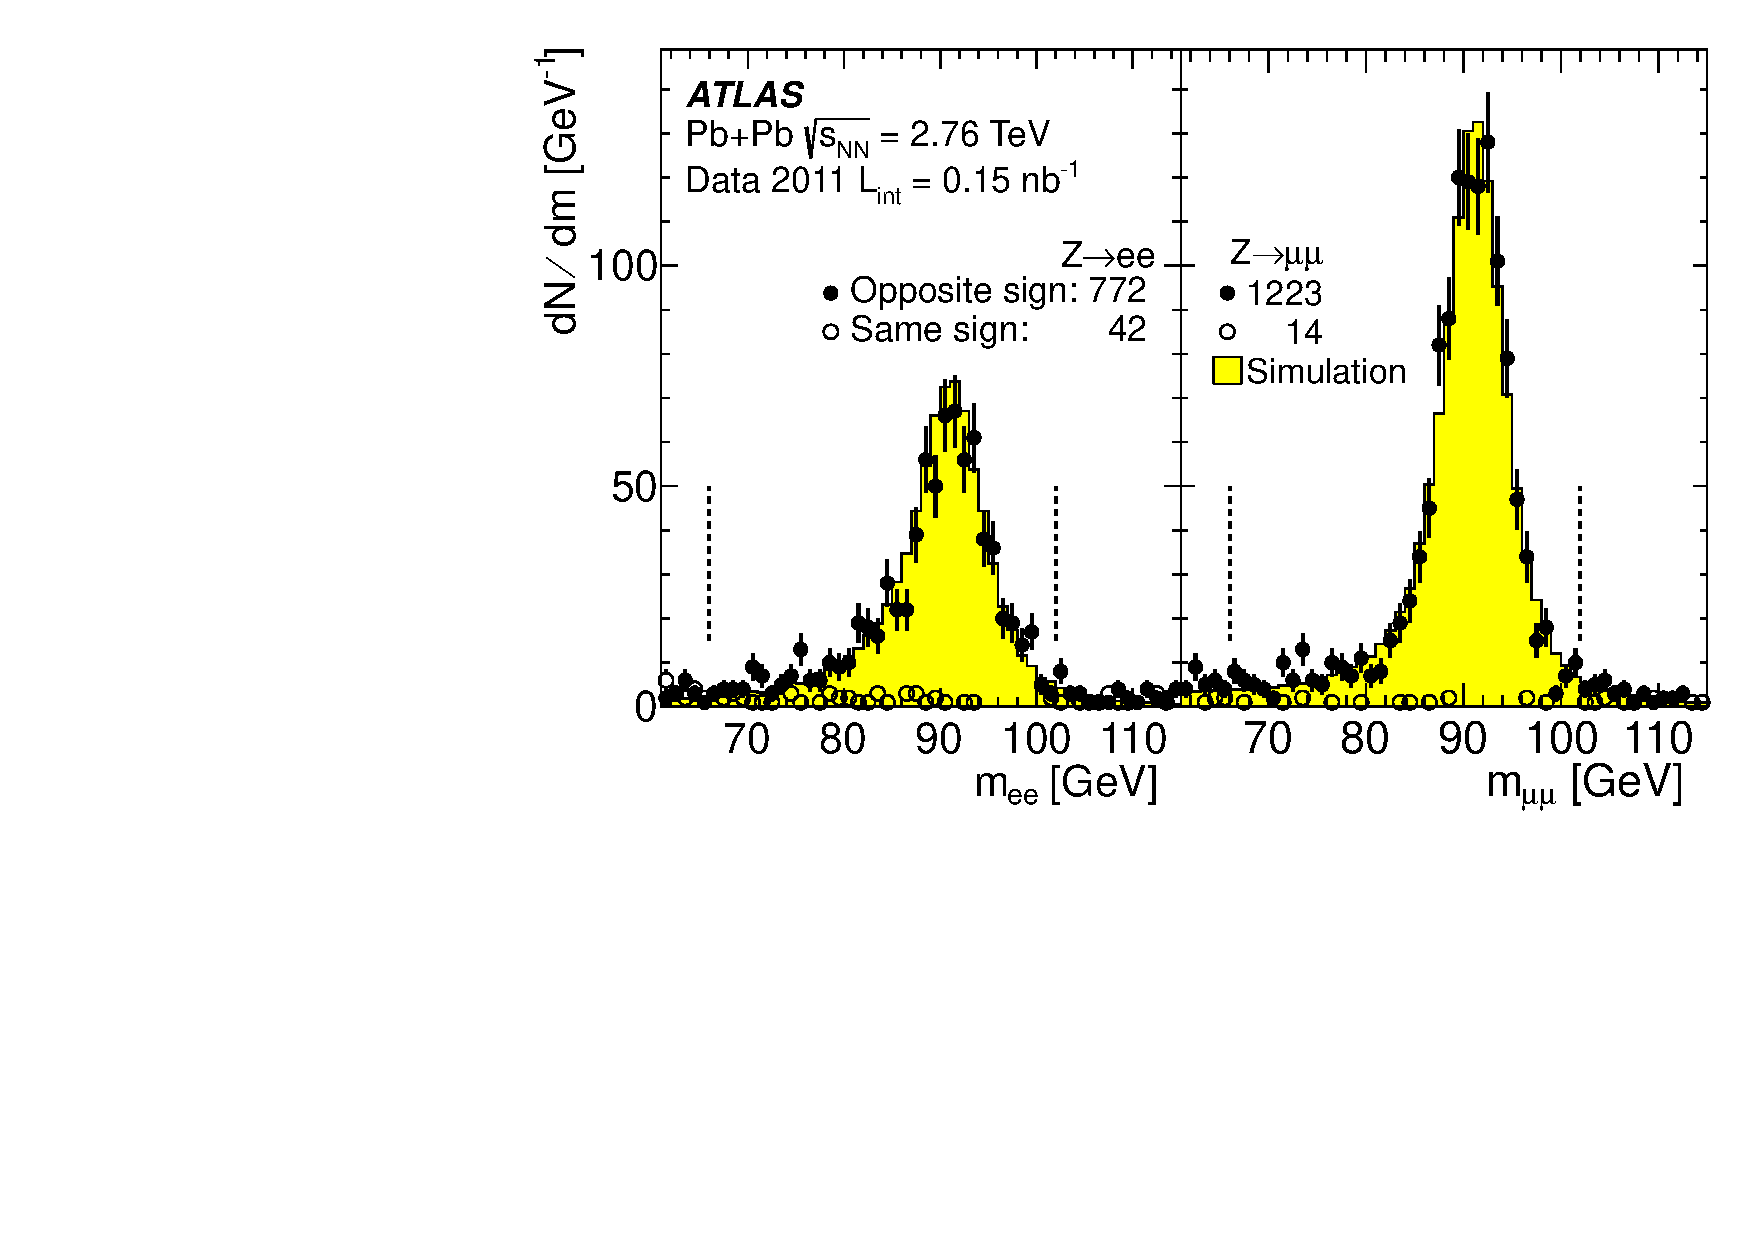
\includegraphics[width=0.49\textwidth]{electroweak_figs/fig_01.pdf}
\caption[]{(left) Single muon spectrum, after selection cuts (right) Dimuon mass spectrum, in electron and muon channels.}
\label{fig:pas:zw}
\end{center}
\end{figure}

\begin{figure}[!htb]
\begin{center}
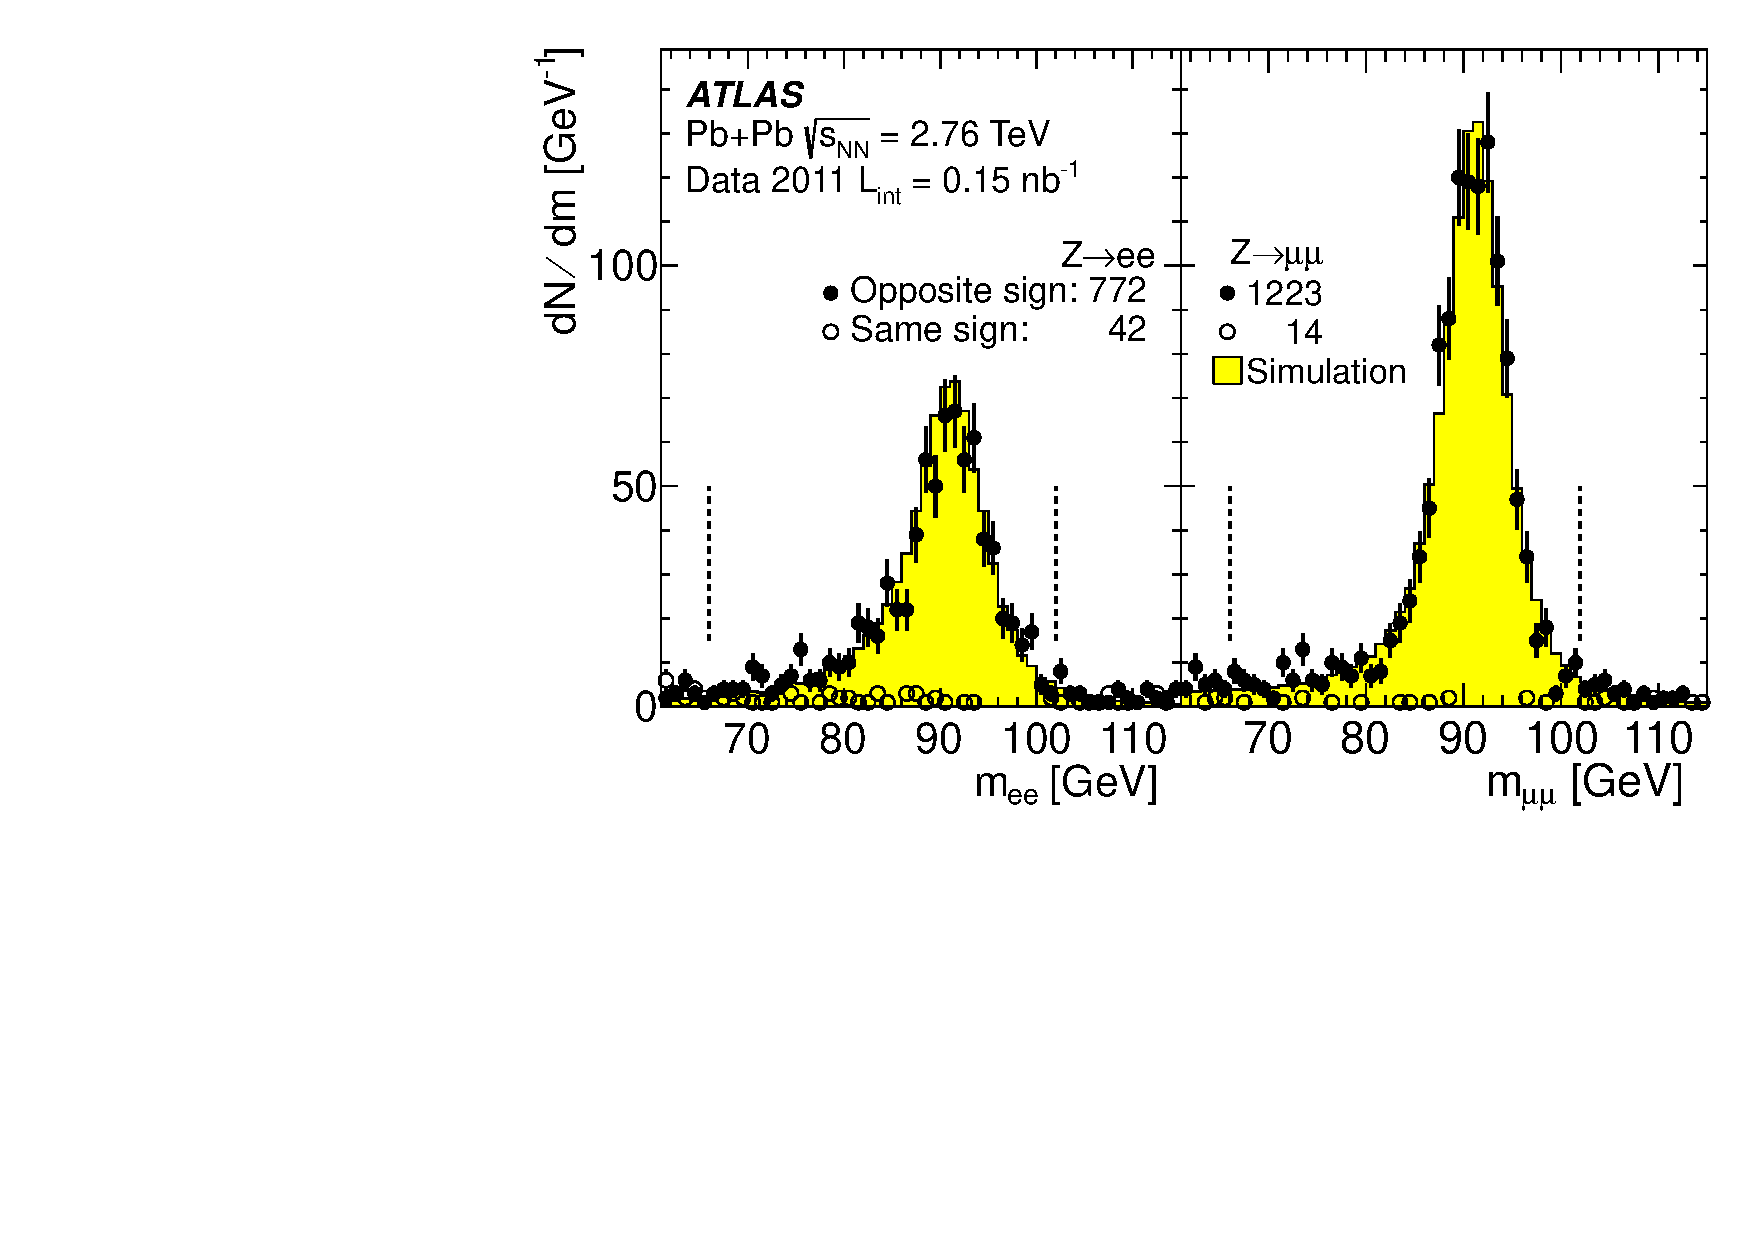
\includegraphics[width=0.49\textwidth]{electroweak_figs/fig_01.pdf}
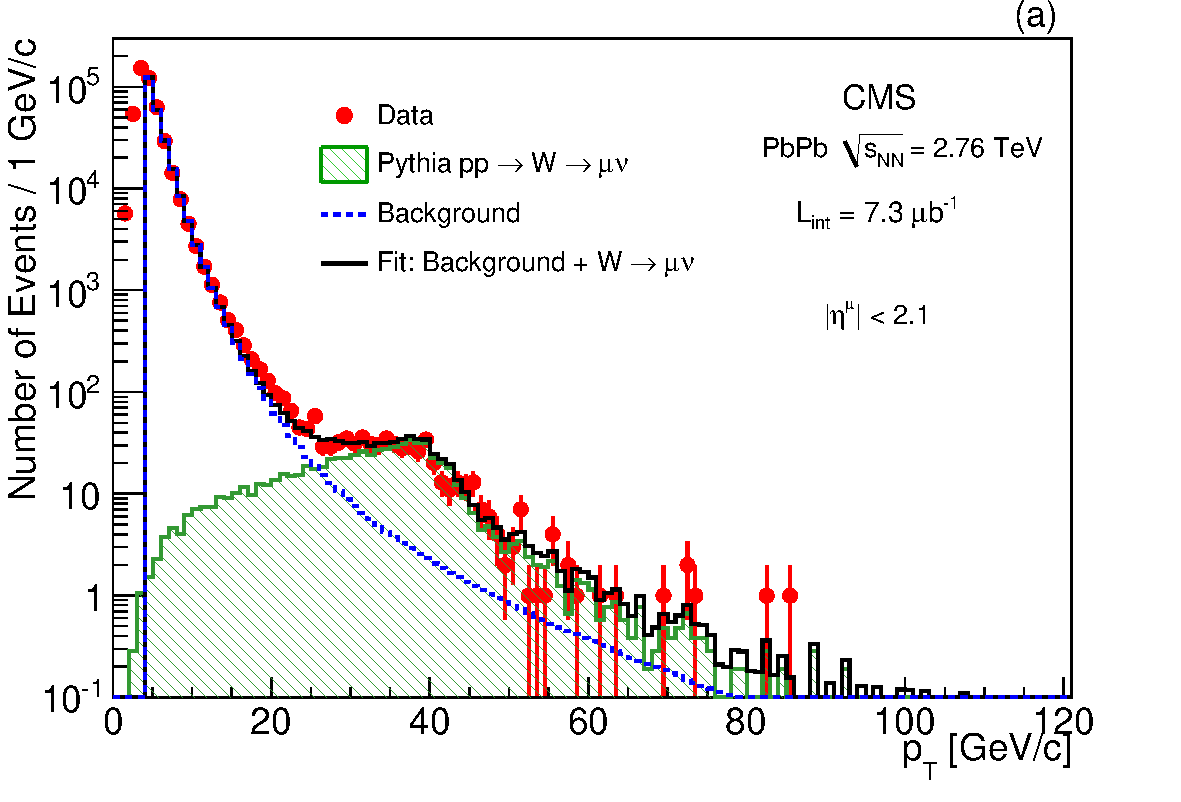
\includegraphics[width=0.49\textwidth]{electroweak_figs/Fig1a.pdf}
\caption[]{(left) Single muon spectrum, after selection cuts (right) Dimuon mass spectrum, in electron and muon channels.}
\label{fig:pas:zw}
\end{center}
\end{figure}

\begin{figure}[!htb]
\begin{center}
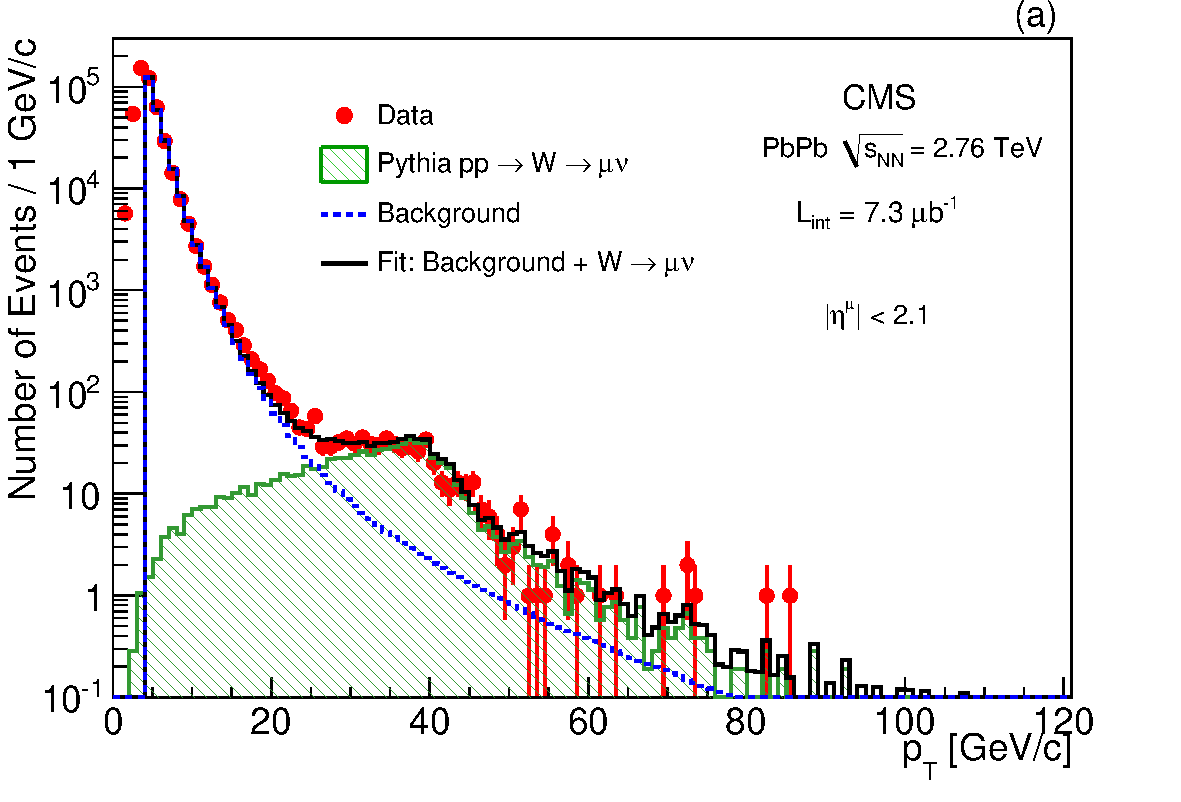
\includegraphics[width=0.49\textwidth]{electroweak_figs/Fig1a.pdf}
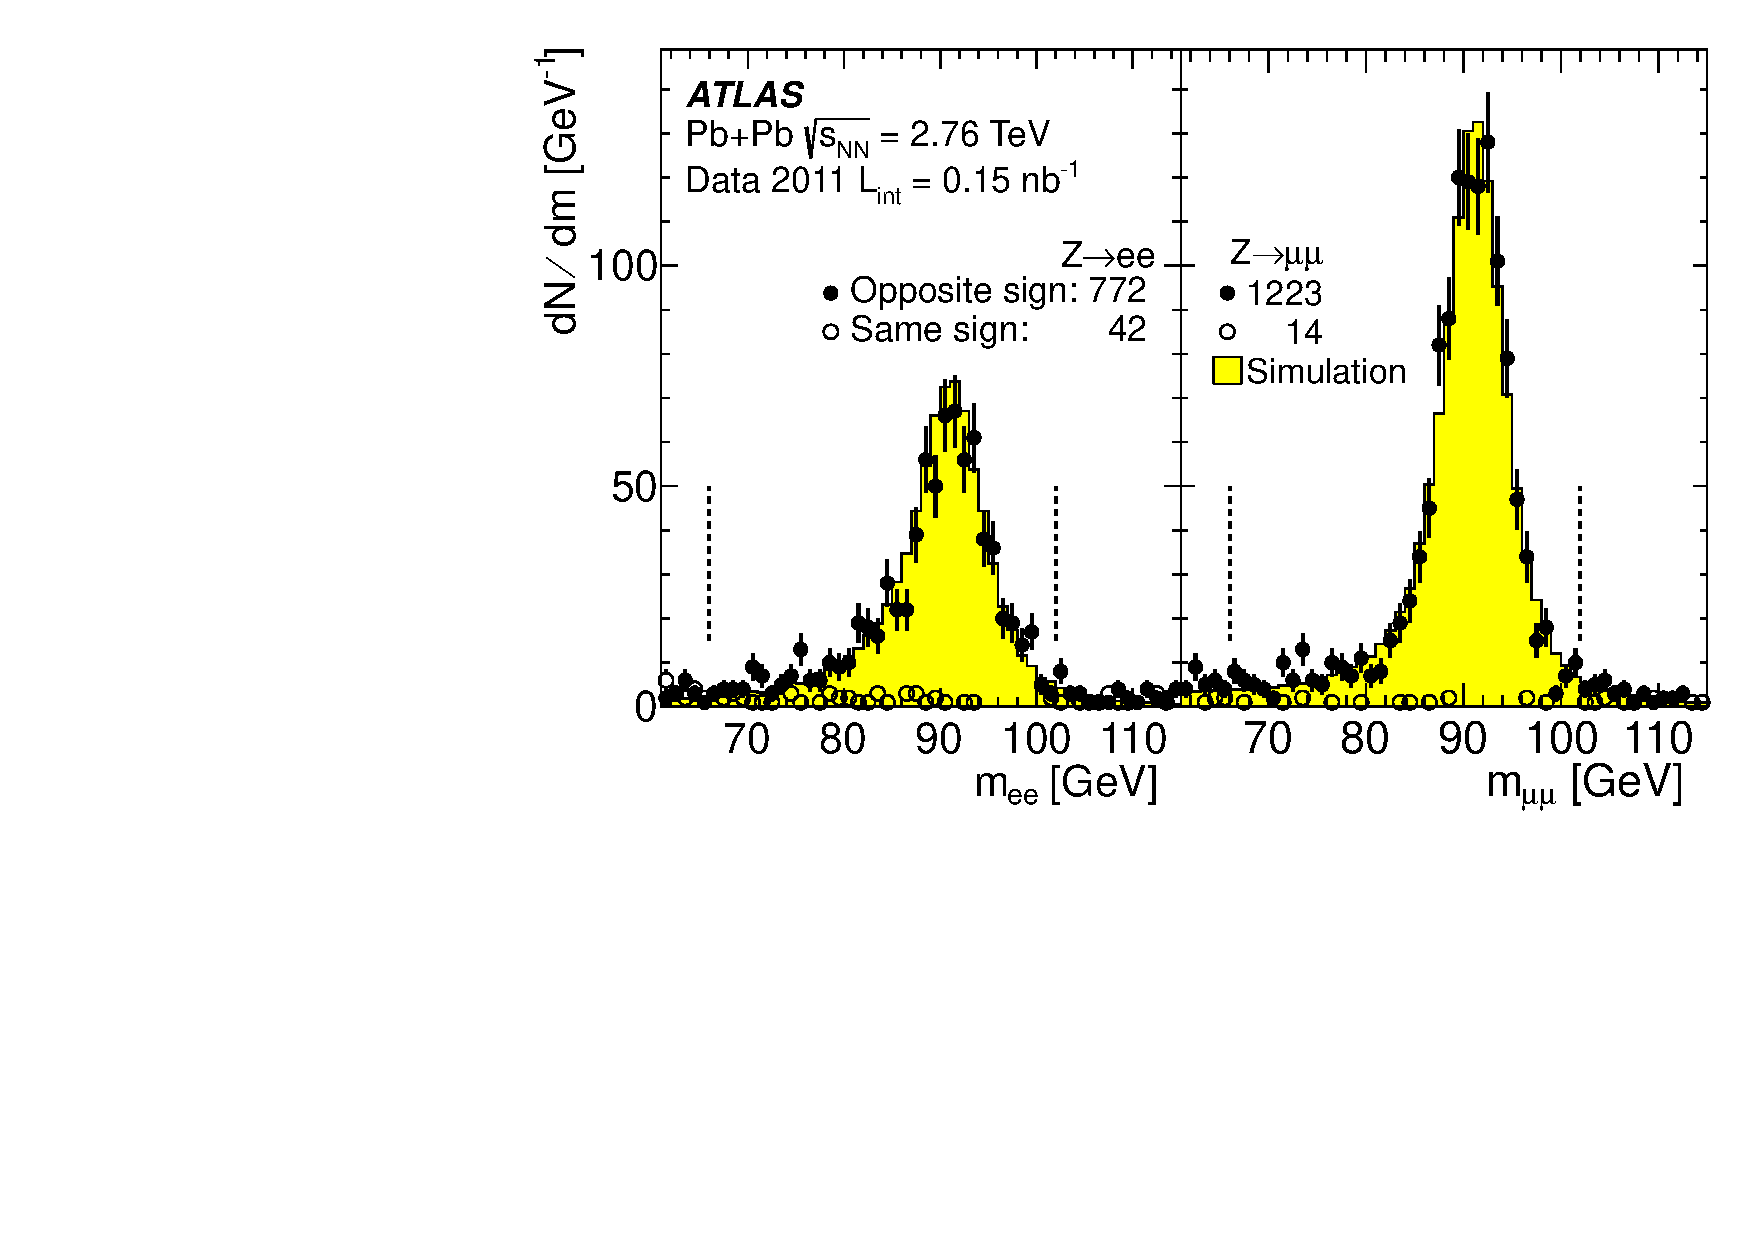
\includegraphics[width=0.49\textwidth]{electroweak_figs/fig_01.pdf}
\caption[]{(left) Single muon spectrum, after selection cuts, from CMS data (right) Dimuon mass spectrum, in electron and muon channels from ATLAS data.}
\label{fig:pas:zw}
\end{center}
\end{figure}

\begin{figure}[!htb]
\begin{center}
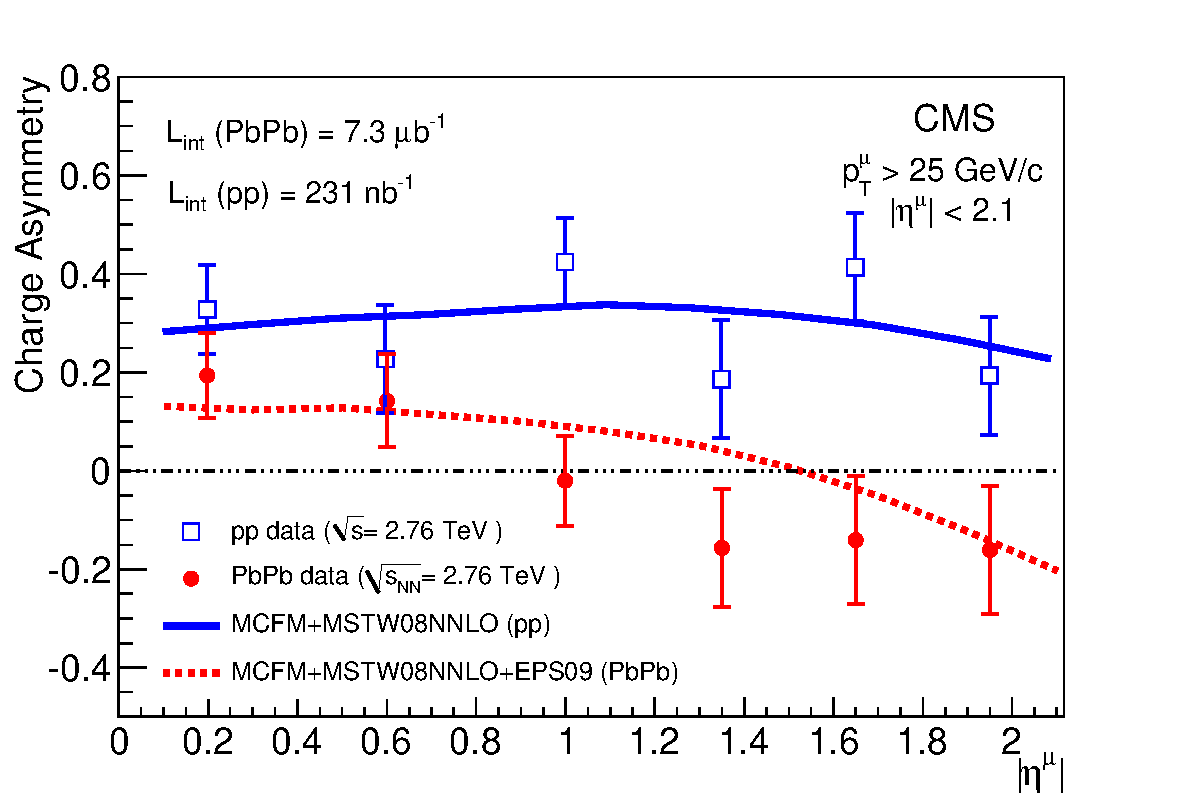
\includegraphics[width=0.49\textwidth]{electroweak_figs/Fig3.pdf}
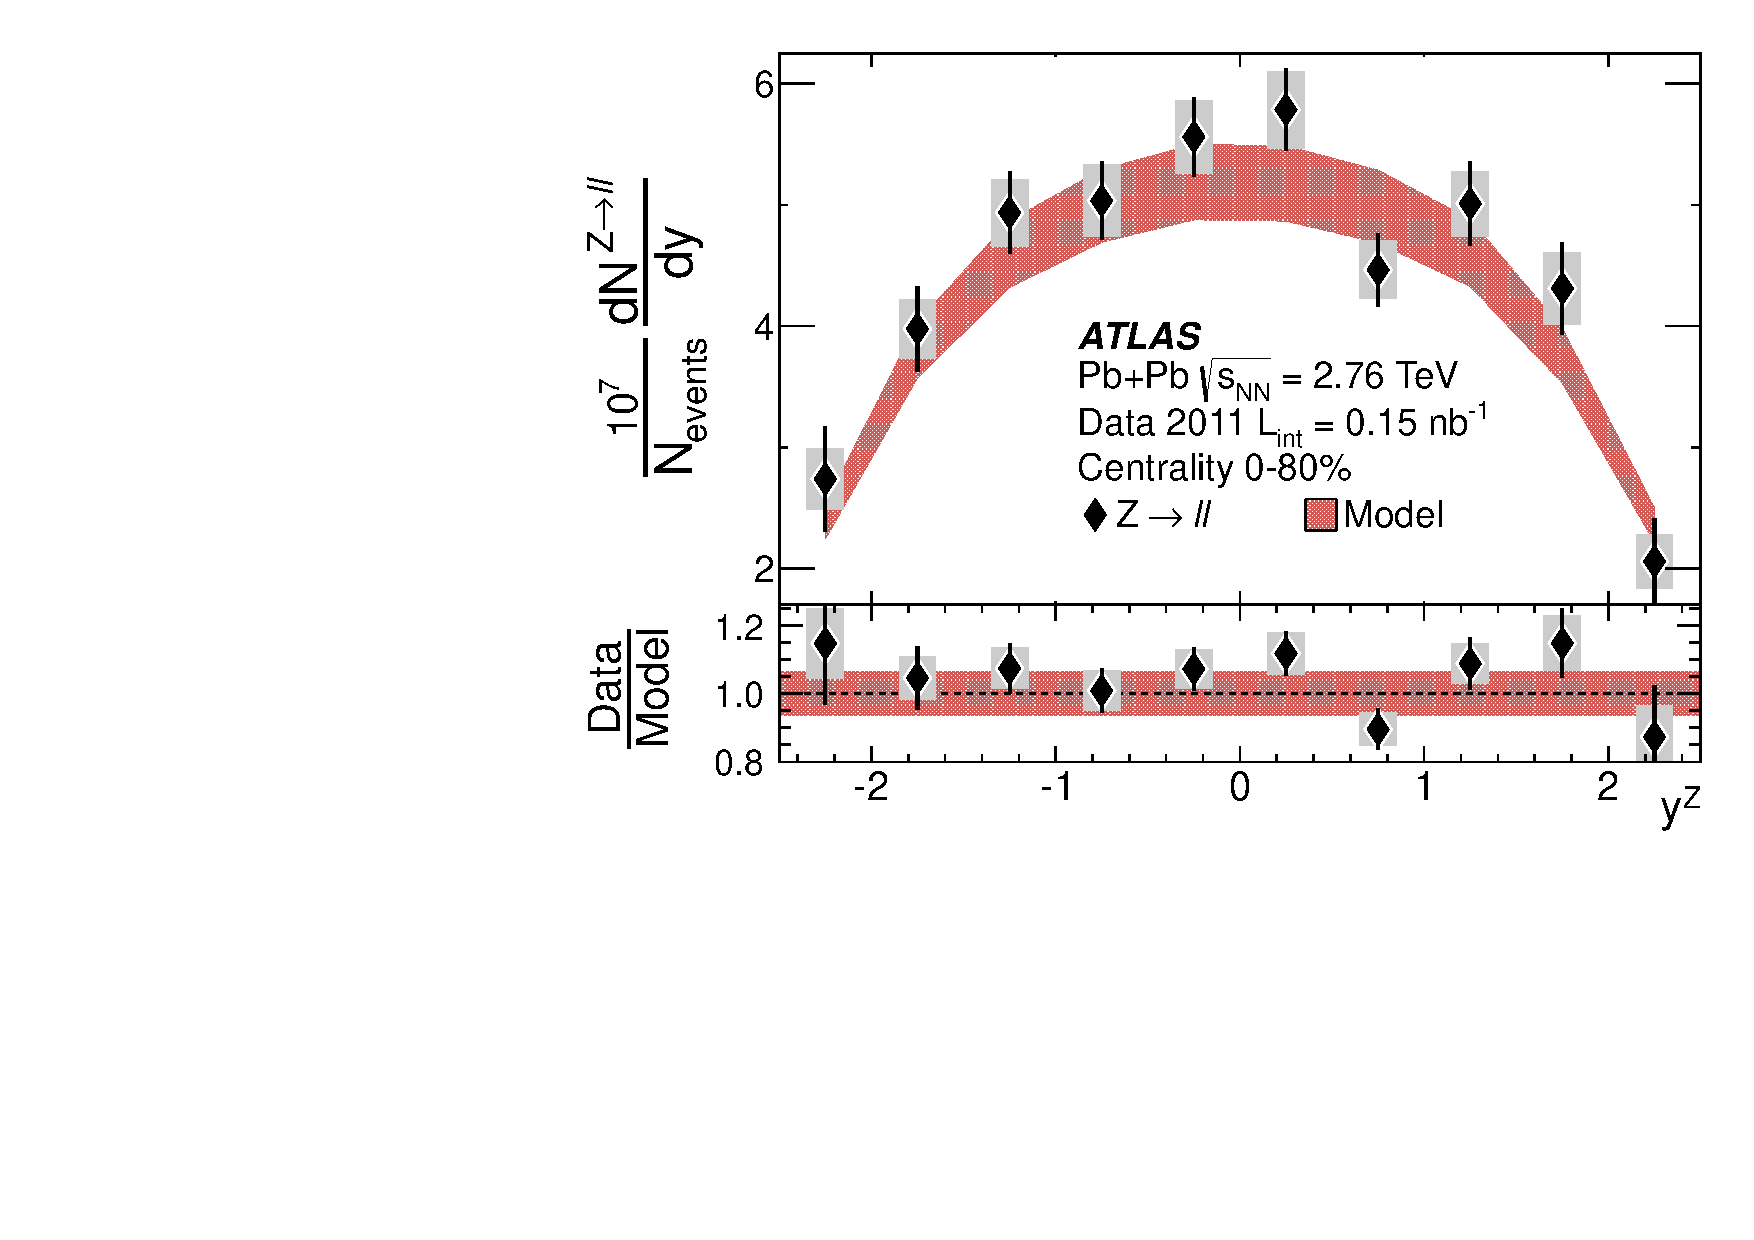
\includegraphics[width=0.49\textwidth]{electroweak_figs/fig_02.pdf}
\caption[]{(left) Charge asymmetry for W candidates, from CMS data (right) Dimuon mass spectrum, in electron and muon channels from ATLAS data.}
\label{fig:pas:zw}
\end{center}
\end{figure}

\begin{figure}[!htb]
\begin{center}
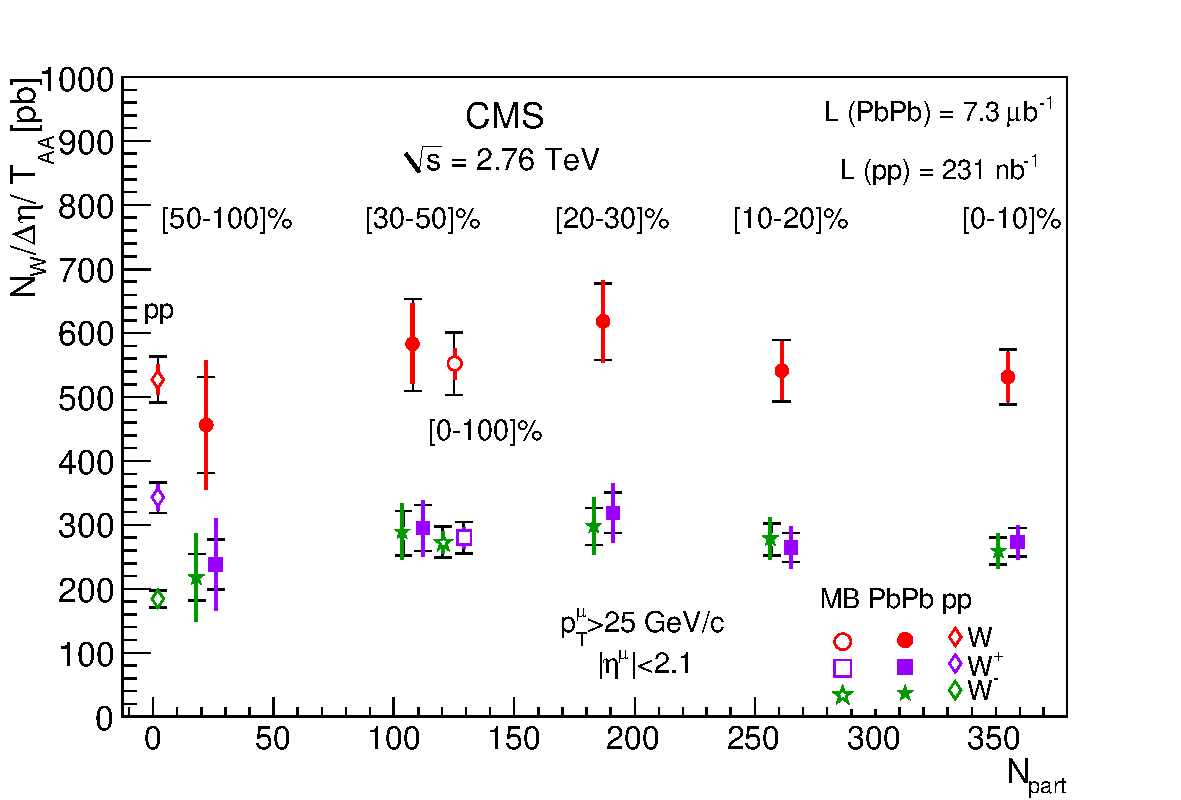
\includegraphics[width=0.49\textwidth]{electroweak_figs/Fig2.pdf}
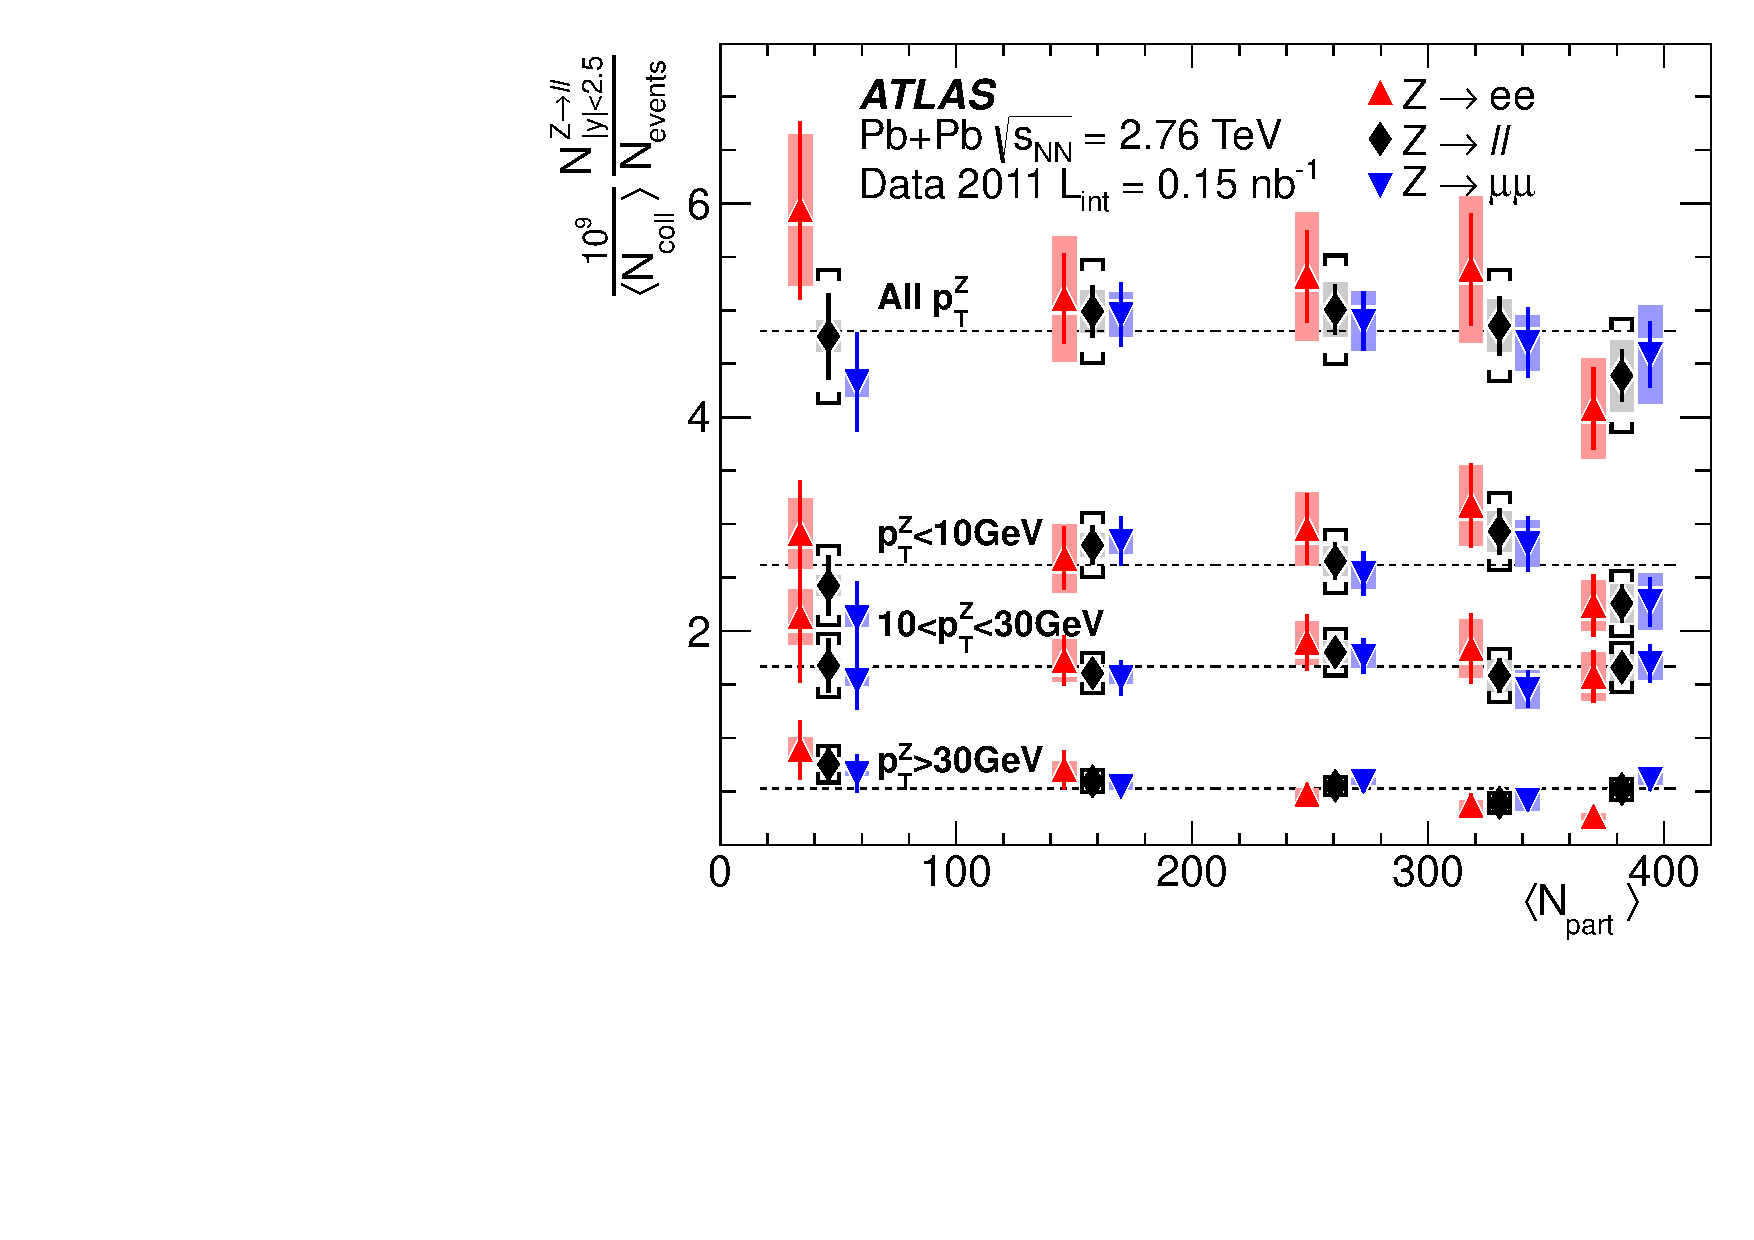
\includegraphics[width=0.49\textwidth]{electroweak_figs/fig_04.pdf}
\caption[]{(left) Yield per collision for W candidates, from CMS data (right) Yield per collision for Z's, in both electron and muon channels from ATLAS data.}
\label{fig:pas:zw}
\end{center}
\end{figure}


\begin{figure}[!htb]
\begin{center}
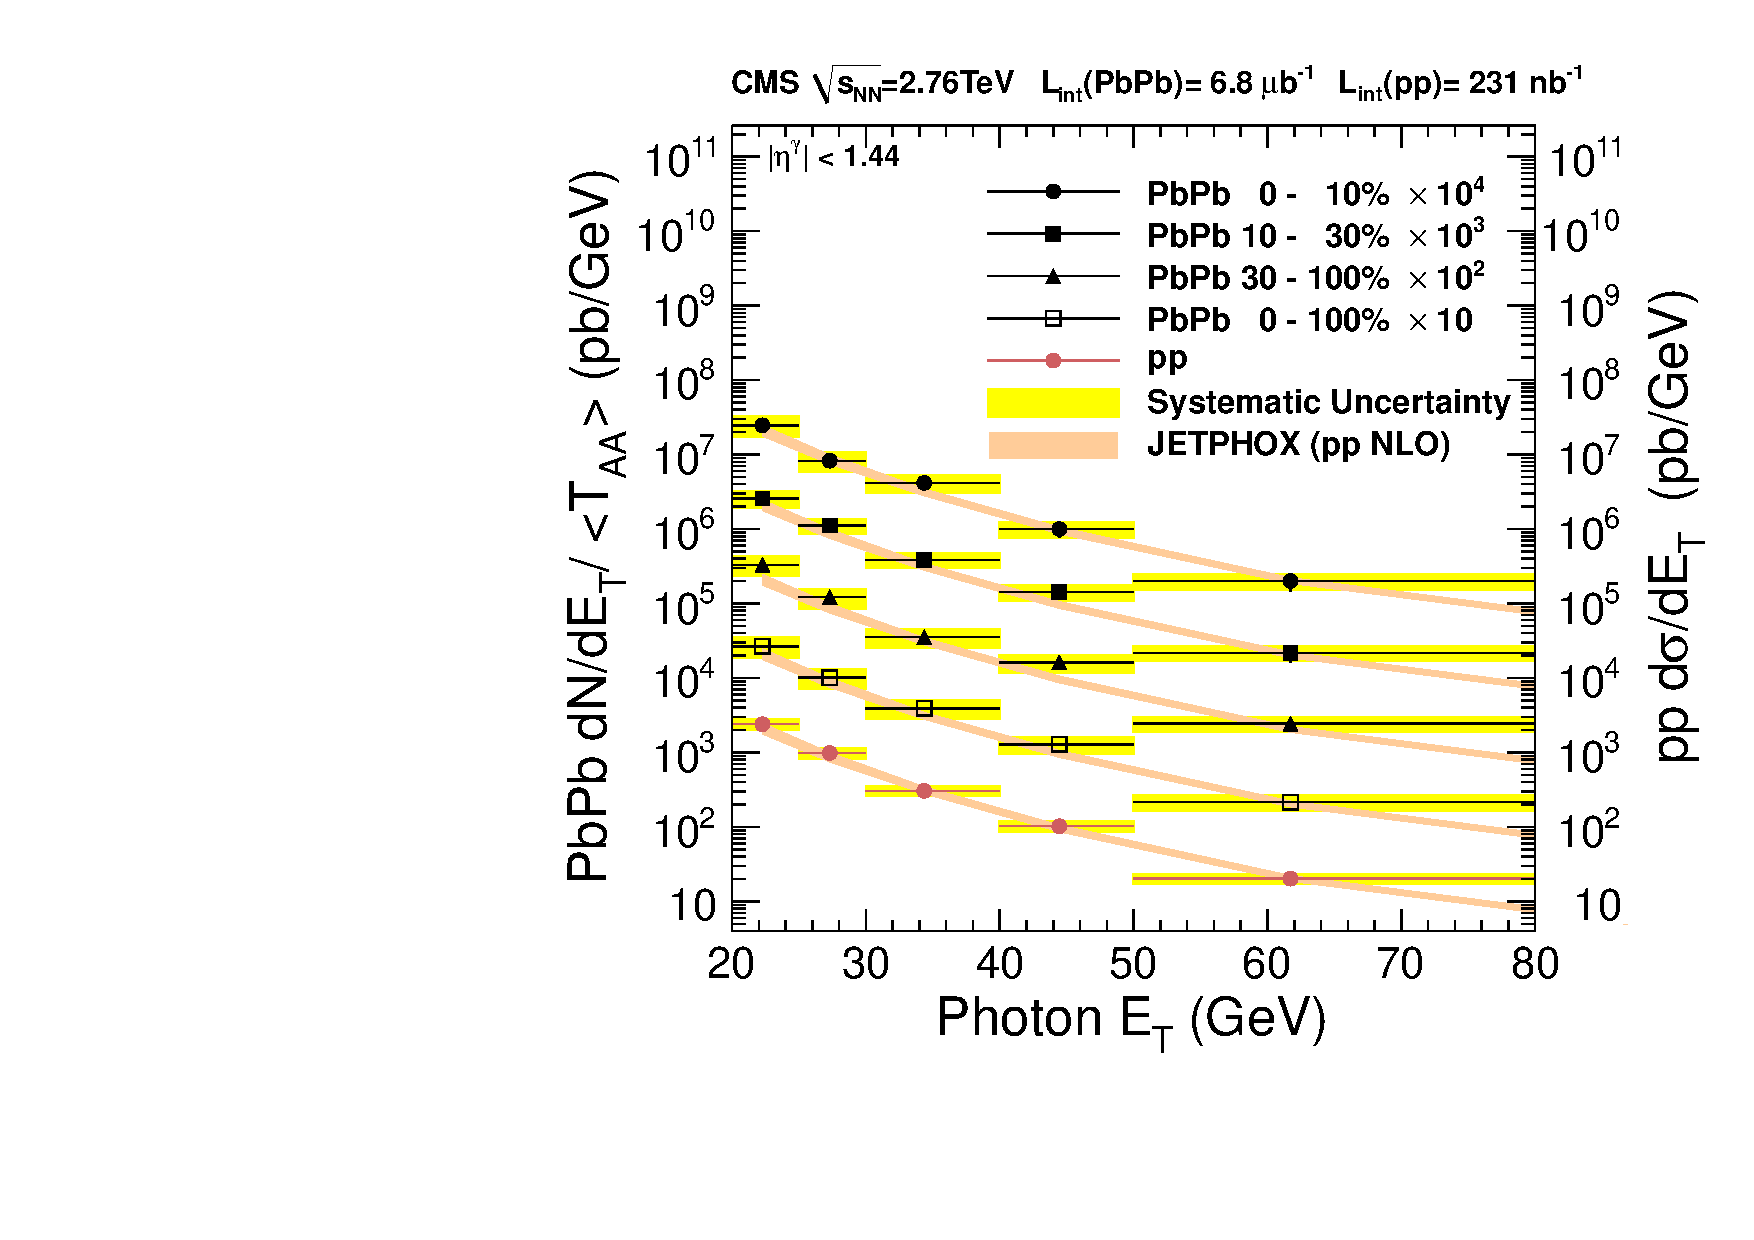
\includegraphics[width=0.49\textwidth]{electroweak_figs/TAAScaling.pdf}
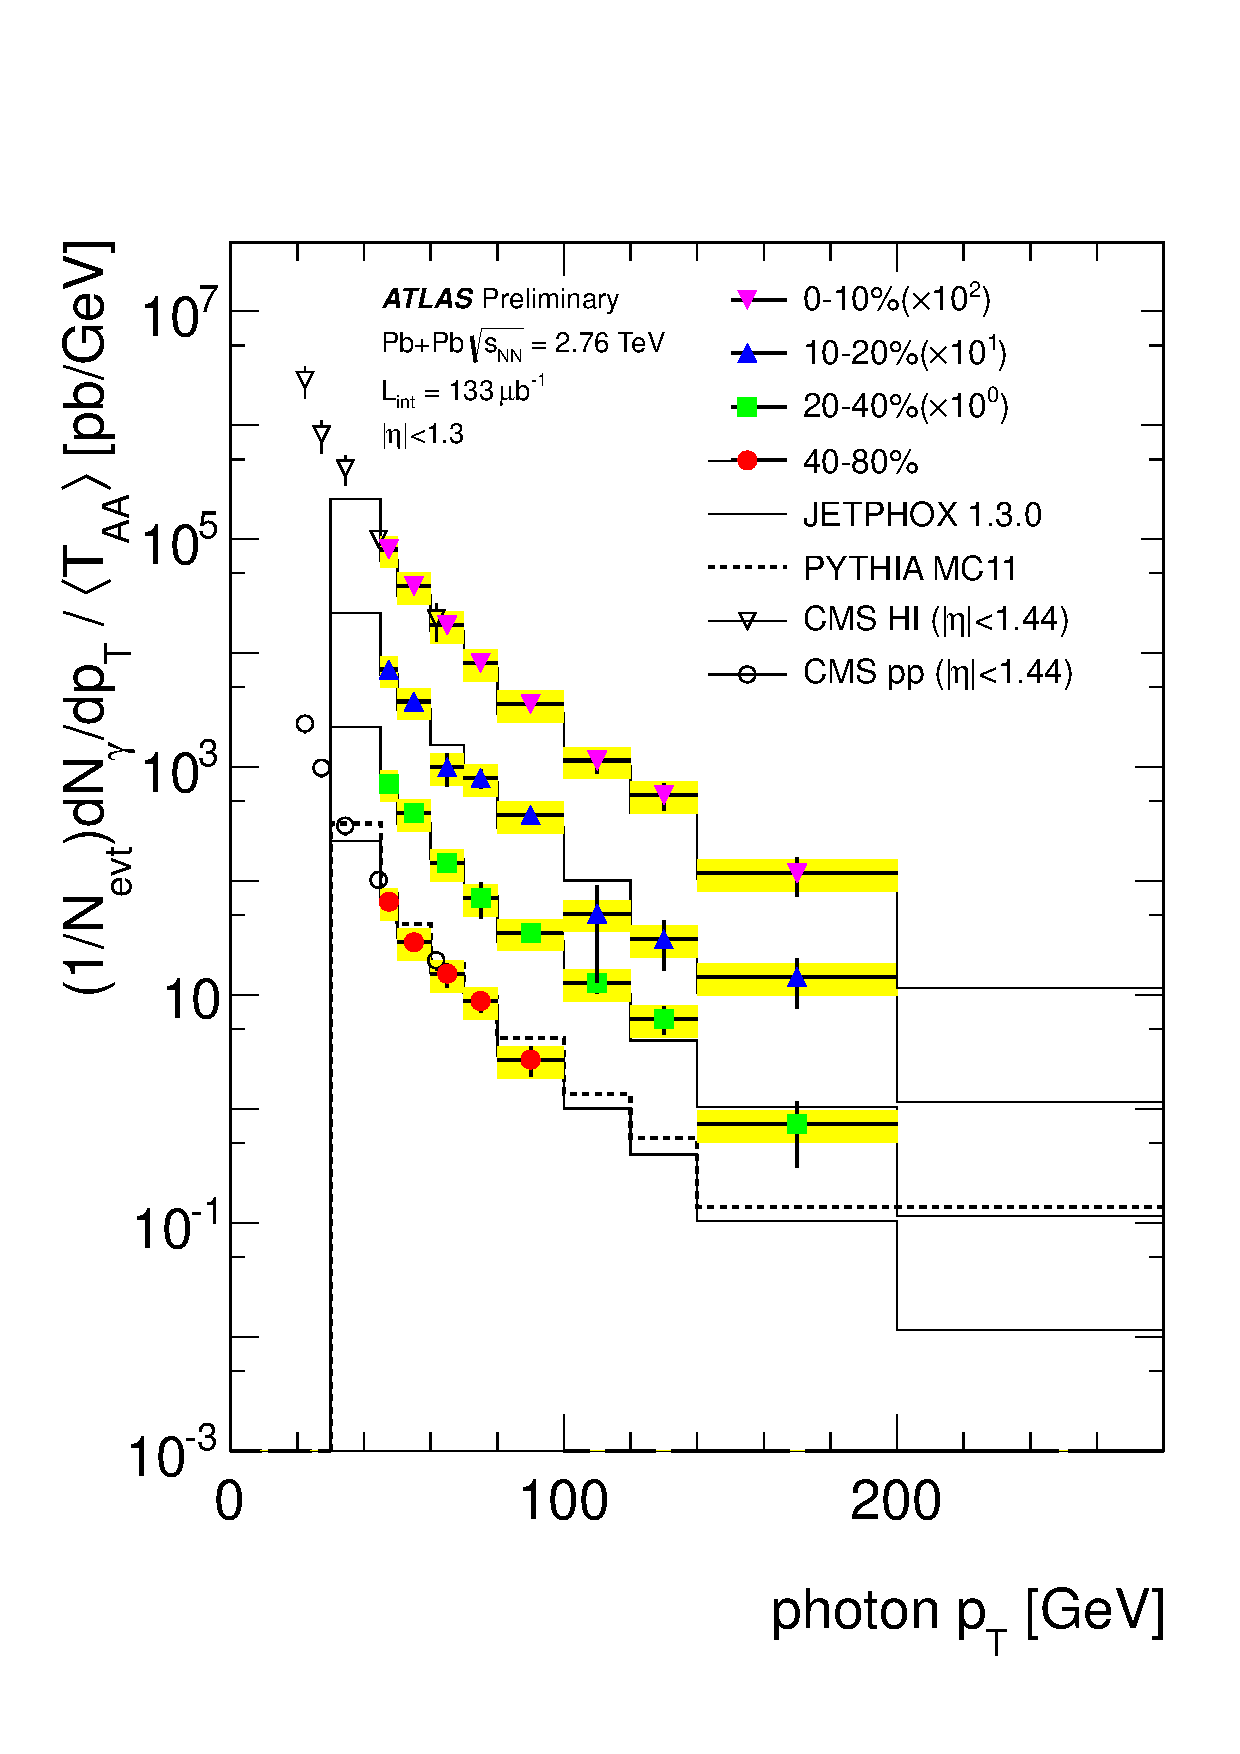
\includegraphics[width=0.49\textwidth]{electroweak_figs/ph_fig_11.pdf}
\caption[]{(left) Photon yields scaled by the mean nuclear thickness function for $|\eta|<1.44$, from CMS data (right) The similar quantity from ATLAS, for $|\eta|<1.3$, from ATLAS data.}
\label{fig:pas:zw}
\end{center}
\end{figure}


